\section{General approach}

In this section, we propose a gneralized approach for performing declarative
static analysis for a multilingual program.

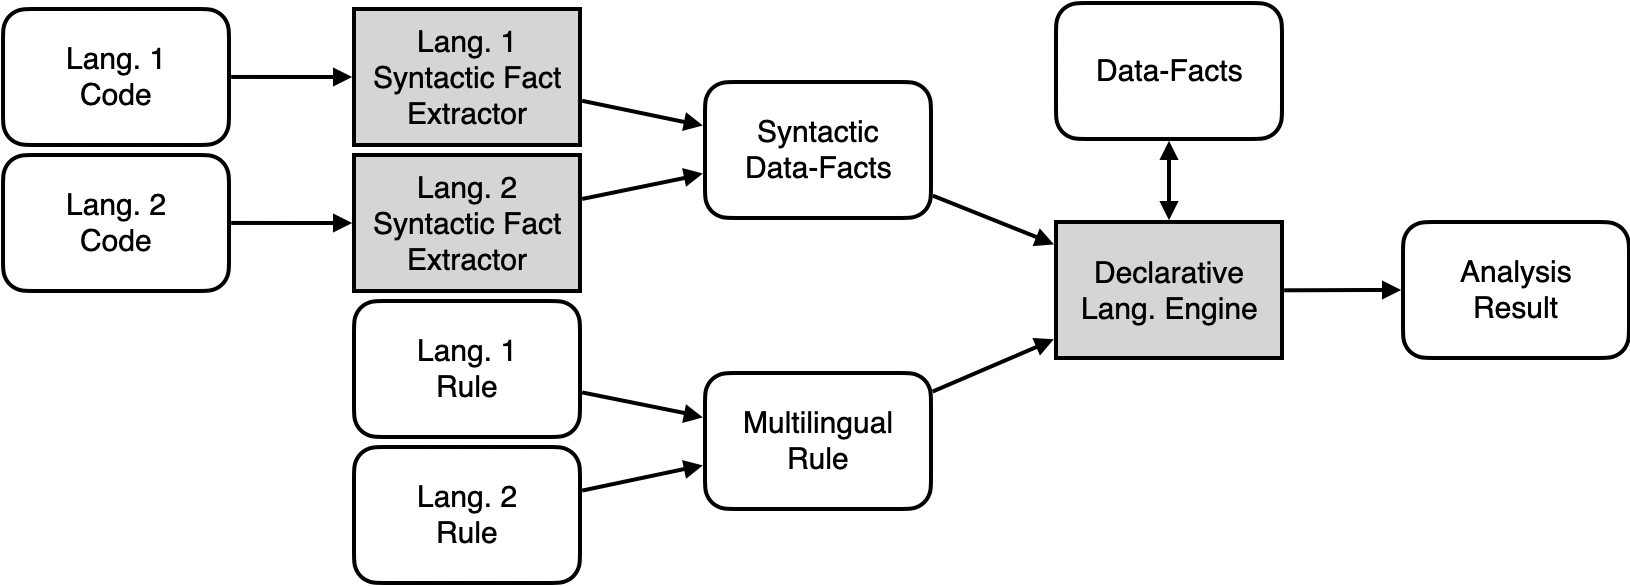
\includegraphics[width=0.5\textwidth]{img/overview}

Above figure illustrate the overview of this approach. The analysis mainly
consists of three steps. First, each language is converted into a syntactic
data-facts. Second, the rule for generating data-facts are defined. Finally,
the declarative language engine is executed with the given data-facts and
rules, giving the analysis result as an output in form of data fact.

\subsection{Syntax of data-fact and rule}

First, we define the syntax of data-fact and rule, which is fairly simple.

\[e := num | string\]
\[df := p(\overline{e})\]
\[r := df :- \overline{(not)? df}\]

e stands for an element, and is either number or string.  df stands for
data-fact, and it is an ordered tuple of elements.  r stands for rule, and it
denotes how one rule can be derived from another data-facts.  It states that
LHS data-fact(the data-fact before the symbol ":-") holds if all RHS data-facts
(data-facts after the symbol ":-") without "not" notation holds, and all RHS
data-facts with "not" notation does not hold.  (? Note that recursion is
permitted, that is, a data-fact can depend on itself.  The exception is the
recursion with odd number of negation, that is, the rule such as "p(x) :- not
p(x)" is not valid. ?)

\subsection{Extracting syntactic data-fact}

The first step is to extract syntactic data-facts from the source code.
The example of syntactic data-facts would be data-facts about certain
AST node, or parent-child relationship between nodes. For example, if we
have the following source code:

1 int x = 42 + 43;

we can define "expr(i, s)" to be a name of data-fact, which is 2-dimensional
tuple of expression id and the expression string represented in source code.
Therefore, we will have the set of expr data-facts: expr(0, "42"), expr(1,
"43"), and expr(2, "42 + 43").  Another example of syntactic fact would be
"subexpr(i, j, k)", which is a 3-dimensional data-fact which states that the
expression with id i has expression with id j as a kth expression. For example,
we can find the rule subexpr(2, 0, 1) and subexpr(2, 1, 2).

The advantage for extracting syntactic data-facts is that once they are extracted,
they can be utilzed easily in any other kind of analysis, since they are basically
also a data-fact that can be simply manipulated by rules.

\subsection{Defining rule}

The next step is defining rules to generate new data-facts on top of know
data-facts, that is, actually implementing the analysis in declrative style.
This setp can be futrher divided into more sub tasks. First thing to do is to
designing the generalized and unified framework for static analysis,
that can incorporate both languages. The second step is to actually fill in
the implementation, for each of the language. The interoperation between two languages
is considered in the final step, where some rules in frameworks are extended
to handle the interoperation between them, while the language-specific implementation itself
needs little modification.

There would be the trade-off between the generality of framework, and the
complexity of implementation. Designing more general and shallow framework
would be easier, yet it would require more detailed implmentaion of the framework. On the other
hand, one can design more language-specific framework which would reduce the
burden of implemenation, but designing a good framework that is suitable for both
languages would be rather challenging.

Let's look at the concrete example of dataflow analysis. First thing we do is
designing the analysis framework, which can be applied to both of the language.
In this framework, the analysis result we want is expressed with the data-fact
of the form of flow(a,b), which means that value of the node a can flow into
node b. flow(a, b) can be defined as transitive closure of a data-fact step(a,
b);

flow(a,b) :- step(a,b) or step(a,c) and flow(c, b)

where the data-fact step(a,b) means that there is a direct flow from node a to b.
Next thing to do is defining rule for the data-fact step for each language.
For example, if a lnaguage has a syntactic data-fact which indicates the assignment
x = val, in form of assign(val, x), then one can define a rule for step to be
step(a, b) :- assign(a,b). The final step is to take the inter operation into account.
A way to pass data in one language into another is via funcction call, which can be
reflected into the rule of step(a,b) :- foreignArgParam(a,b,i), where foreignArgParam(a,b,i)
is the data-fact that indicates a is an i-th argument of a foreign function call to a
function, whoose i-th argument is b.

An alternative to this framework, is defining a more fine-grained rule for step:
Assuming that both target languages have function call and field access, step (a,b) can be

step(a,b) :- localStep(a, b) or functionInStep(a, b) or functionOutStep(a, b)
or filedReadStep(a, b) or fieldWriteStep(a, b)

as a part of the framework. Here, localStep represents any flows that do not
envolve function call or field access.  Example would be assigning to a
variable, or simple def-use pattern.  functionInStep and functionOutStep are
used for flows envolving function calls, such as flow from argument to
parameter or flows regarding return statement.  fieldReadStep and
fieldWriteStep are predicates for field access. Then, the implementation of
each framework, and the rules for inter-operation, can be written on top of
this framework. This framework has the advantage of being modular, and rule for
each framework data-facts being simpler, but desigining this framework would
require the designer to verify if this design is indeed appropriate one, i.e.,
there is no other possible steps.


\subsection{Evaluating rules}

The final step is to simply evaluate the defined rules, with the given data-facts.
By evaluating the rules, we mean that finding all possible data-facts that
can be derived. The rules are ususally evaluated in bottom-up and
modular manner, that is, each rule is evaluated one-by-one, after every rule
it depends on is evaluated.


